\chapter{Thermoelasticity in port-Hamiltonian form}

\epigraph{Eh bien, mon ami, la terre sera un jour ce cadavre refroidi. Elle deviendra inhabitable et sera inhabitée comme la lune, qui depuis longtemps a perdu sa chaleur vitale.}{\textit{Vingt mille lieues sous les mers\\
Jules Verne}}
\minitoc
 
\lettrine{\color{theme}{T}}hermoelasticity is the study of deformable bodies undergoing thermal excitations. It is a clear example of a multiphysics phenomenon since the heat transfer and elastic vibrations within the body mutually interact. In this chapter, a linear model of thermoelasticity is obtained under the pH formalism. Each physics is described separately and the final system is obtained considering a power-preserving interconnection of two pHs.

\begin{comment}
The first work on this discipline dates back to \cite{duhamel1837}, but it was only more than a century later, thanks to the paper of Biot \cite{biot1956thermoelasticity}, that research on this topic received a new impulse.
\end{comment}

\section{Port-Hamiltonian linear coupled thermoelasticity}\label{sec:phthel}
In this section, a pH formulation of heat transfer is first introduced. The classical model of thermoelasticity is then recalled. The same model is found by interconnecting the heat equation and the linear elastodynamics problem seen as pHs. It is shown that the interconnection preserves a quadratic functional that plays the role of a fictitious energy. The resulting system is dissipative  with respect to this functional. The construction makes use of the intrinsic modularity of pHs \cite{kurula2010}.

\subsection{The heat equation as a pH descriptor system}\label{sec:phheat}
Consider the heat equation in a bounded connected set $\Omega \subset \mathbb{R}^d, \, d=\{1,2,3\}$, describing the evolution of the temperature field $T(\bm{x}, t)$
\begin{equation}\label{eq:heatEq}
\rho c_\epsilon \diffp{T}{t} = k \Delta T + r_Q, \qquad \quad \bm{x} \in \Omega,
\end{equation}
where $\rho,\, c_\epsilon,\, k,\, r_Q$ are the mass density, the specific heat density at constant strain, the thermal diffusivity and an heat source. Symbol $\Delta$ denotes the Laplacian in $\mathbb{R}^d$.The Dirichlet and Neumann condition of this problem are 
\begin{equation*}
	\begin{aligned}
	T \text{ known on } \Gamma_D^T, \qquad \text{Dirichlet condition}, \\
	-k \, \grad T \cdot \bm{n} \text{ known on } \Gamma_N^T, \qquad \text{Neumann condition},
	\end{aligned}
\end{equation*}
where a partition of the boundary $\partial \Omega = \Gamma_D^T \cup \Gamma_N^T$ has been considered. This model can be put in pH form by means of a canonical interconnection structure. An algebraic relationship that describes the Fourier law has to be incorporated in the model (cf. \cite[Chapter 2]{kotyczka2019numerical}). Here, a differential-algebraic formulation is exploited to obtain the same system. \\

Let $T_0$ be a constant reference temperature (the introduction of this variables is instrumental for coupled thermoelasticity). The functional 
\begin{equation*}
	H_T = \frac{1}{2} \int_\Omega \rho c_\epsilon T_0 \left(\frac{T-T_0}{T_0} \right)^2 \d\Omega
\end{equation*} 
has the physical dimension of an energy and represents a Lyapunov functional of this system. Even though it does not represent the internal energy, it has some important properties. Select as energy variable 
\begin{equation*}
\alpha_T := \rho c_\epsilon (T-T_0),
\end{equation*}
whose corresponding co-energy is 
\begin{equation*}
	e_T := \diffd{H_T}{\alpha_T} = \frac{\alpha_T}{\rho c_\epsilon T_0} = \frac{T-T_0}{T_0} =: \theta.
\end{equation*}
Introducing the heat flux $\bm{j}_Q := -k \grad T$ as additional variable, the heat equation \eqref{eq:heatEq} is equivalently reformulated as
\begin{equation}\label{eq:phsysHeat}
\begin{aligned}
\begin{bmatrix}
1 & 0 \\
\bm{0} & \bm{0} \\
\end{bmatrix}
\diffp{}{t}
\begin{pmatrix}
\alpha_T \\
\bm{j}_Q \\
\end{pmatrix} &= 
\begin{bmatrix}
0 & -\div \\
-\grad & -(T_0 k)^{-1} \\
\end{bmatrix}
\begin{pmatrix}
e_T \\
\bm{j}_Q \\
\end{pmatrix} + 
\begin{bmatrix}
1 \\
\bm{0} \\
\end{bmatrix} u_T, \\
y_T &= \begin{bmatrix}
1 & \bm{0} \\
\end{bmatrix} \begin{pmatrix}
e_T \\
\bm{j}_Q \\
\end{pmatrix}.
\end{aligned}
\end{equation}
with $u_T:=r_Q$ and $y_T$ represents the corresponding power-conjugated variable. In matrix notation, it is obtained
\begin{equation}
\begin{aligned}
\mathcal{E}_T \partial_{t} \bm{\alpha}_T  &= \left(\mathcal{J}_T - \mathcal{R}_T \right)\bm{e}_T + \mathcal{B}_{T}\, u_T, \\
y_d &= \mathcal{B}_{T}^* \, \bm{e}_T
\end{aligned}
\end{equation}
where $\bm{\alpha}_T = (\alpha_T,\ \bm{j}_Q), \; \bm{e}_T = (e_T,\ \bm{j}_Q)$ and
\begin{equation*}
\mathcal{E}_T = \begin{bmatrix}
1 & 0 \\
\bm{0} & \bm{0} \\
\end{bmatrix}, \quad
\mathcal{J}_T = \begin{bmatrix}
0 & -\div \\
-\grad & \bm{0} \\
\end{bmatrix}, \quad 
\mathcal{R}_T = \begin{bmatrix}
0 & 0 \\
\bm{0} & (T_0 k)^{-1} \\
\end{bmatrix}, \quad
\mathcal{B}_T = \begin{bmatrix}
1 \\
\bm{0} \\
\end{bmatrix}.
\end{equation*}
The system is an example of pH descriptor system (cf. \cite{beattie2018linear} for the finite dimensional case). The Hamiltonian reads 
\begin{equation}\label{eq:hamHeat}
	H_T = \frac{1}{2}\int_\Omega \bm{e}_T \cdot \mathcal{E}_T\bm{\alpha}_T \d\Omega.
\end{equation}
The power rate is then deduced
\begin{equation}\label{eq:enrateHeat}
\begin{aligned}
\dot{H}_T &= \int_\Omega \bm{e}_T \cdot \mathcal{E}_T\, \partial_t \bm{\alpha}_T \d\Omega, \\
		&= \int_\Omega \bm{e}_T \cdot \left\{(\mathcal{J}_T-\mathcal{R}_T) \bm{e} + \mathcal{B}_T u_T \right\} \d\Omega, \\
		&= \int_\Omega u_T \, y_T \d\Omega -\int_\Omega \left(e_T \div \bm{j}_Q + \bm{j}_Q \grad e_T + \frac{\norm{\bm{j}_Q}^2}{k T_0} \right) \d\Omega, \\
		&\le \int_\Omega u_T \, y_T \d\Omega -\int_{\partial\Omega} e_T \ \bm{j}_Q \cdot \bm{n} \d{S}.
\end{aligned}
\end{equation}
This choice of Hamiltonian allows retrieving the classical boundary conditions and leads to a dissipative system. Other formulations, based on an entropy or internal energy functionals, are possible for the heat equation \cite{duindam2009,serhani2019modeling}. These provide an accrescent or a lossless system. Unfortunately these formulations are non linear and their discretization is a difficult task \cite{serhani2019discretization}. 


\subsection{Classical thermoelasticity}
The derivation of the classical theory of thermoelasticity is not carried out here. The reader may consult in \cite[Chapter 1]{hetnarski2009thermal} or \cite[Chapter 8]{abeyaratne2012notes} for a detailed discussion on this topic. 

Consider a bounded connected set $\Omega \subset \mathbb{R}^d, \, d=\{1,2,3\}$. The classical equations for linear fully-coupled thermoelasticity for an isotropic thermoelastic material are \cite{biot1956thermoelasticity,carlson1973}
\begin{equation}\label{eq:sysThElas}
\begin{aligned}
\displaystyle \rho \diffp[2]{\bm{u}}{t} &= \Div(\bm{\Sigma}_{ET}) , \\
\displaystyle \rho c_\epsilon \diffp{T}{t} &= -\div(\bm{j}_Q) - \mathcal{C}_\beta \cddot \displaystyle\diffp{\bm{\varepsilon}}{t}, \\
\bm{\Sigma}_{ET} &= \bm{\Sigma}_E + \bm{\Sigma}_{T}, \\
\bm{\Sigma}_E &= 2\mu \bm{\varepsilon} + \lambda \Tr(\bm{\varepsilon}) \bm{I}_{d\times d}, \\
\bm{\Sigma}_T &= - \mathcal{C}_\beta \theta,  \\
\bm{\varepsilon} &= \Grad(\bm{u}), \\
\bm{j}_Q &= -k \, \grad T.
\end{aligned}
\end{equation}
For simplicity  the coupling term
\[\mathcal{C}_\beta:=T_0 \beta(2\mu + d \lambda)\bm{I}_{d\times d} \]
has been introduced. Field $\bm{u}$ is the displacement, $\bm{\varepsilon}$ is the infinitesimal strain tensor, $\bm{\Sigma}_E, \bm{\Sigma}_T$ are the stress tensor contribution due to mechanical deformation and a thermal field. Coefficients $\lambda,\, \mu$ are the Lam\'e parameters,  and $\beta$ the thermal expansion coefficient. Given a partition of the boundary $\partial \Omega = \Gamma_D^E \cup \Gamma_N^E = \Gamma_D^T \cup \Gamma_N^T$ for the elastic and thermal domain. The general boundary conditions read (see Fig. \ref{fig:bc_TherElas2D})
\begin{equation}
\begin{aligned}
\bm{u} \text{ known on } \Gamma_D^E \times (0, +\infty), \\
\bm{\Sigma}_{ET} \cdot \bm{n} \text{ known on } \Gamma_N^E \times (0, +\infty), 
\end{aligned} \qquad
\begin{aligned}
T \text{ known on } \Gamma_D^T \times (0, +\infty), \\
\bm{j}_Q \cdot \bm{n} \text{ known on } \Gamma_N^T \times (0, +\infty).
\end{aligned}
\end{equation}
\begin{figure}[tb]
	\centering
	\includegraphics[width=0.5\textwidth]{part_2/bc_TherElas2D.eps}
	\caption{Boundary conditions for the thermoelastic problem.}
	\label{fig:bc_TherElas2D}
\end{figure}
In the following section an equivalent system is constructed by interconnecting the heat equation and the elastodynamics system in a structured manner.

\subsection{Thermoelasticity as two coupled pHs}

Consider again the equation of elasticity on $\Omega \subset \mathbb{R}^d, \, d =\{1, 2, 3\}$ (cf. Eq. \eqref{eq:phsysElas}), together with a distributed input $\bm{u}_E$ that plays the role of a distributed force
\begin{equation}
\begin{aligned}
\diffp{}{t}
\begin{pmatrix}
\bm{\alpha}_v \\
\bm{A}_{\varepsilon} \\
\end{pmatrix} &= 
\begin{bmatrix}
\bm{0} & \Div \\
\Grad & \bm{0} \\
\end{bmatrix}
\begin{pmatrix}
\bm{e}_v \\
\bm{E}_{\varepsilon} \\
\end{pmatrix} + 
\begin{bmatrix}
\bm{I}_{d\times d} \\
\bm{0} \\
\end{bmatrix}\bm{u}_E, \\
\bm{y}_E &= \begin{bmatrix}
\bm{I}_{d\times d} & \bm{0} \\
\end{bmatrix}
\begin{pmatrix}
\bm{e}_v \\
\bm{E}_{\varepsilon}
\end{pmatrix},
\end{aligned}
\end{equation}
with Hamiltonian  
\[
H_E = \energy{\bm{\alpha}_v \cdot \bm{e}_v + \bm{A}_{\varepsilon} \cddot \bm{E}_{\varepsilon}}.
\]
Recall the pH formulation of the heat equation \eqref{eq:phsysHeat}
\begin{equation}
\begin{aligned}
\begin{bmatrix}
1 & 0 \\
\bm{0} & \bm{0} \\
\end{bmatrix}
\diffp{}{t}
\begin{pmatrix}
\alpha_T \\
\bm{j}_Q \\
\end{pmatrix} &= 
\begin{bmatrix}
0 & -\div \\
-\grad & -(T_0 k)^{-1} \\
\end{bmatrix}
\begin{pmatrix}
e_T \\
\bm{j}_Q \\
\end{pmatrix} + 
\begin{bmatrix}
1 \\
\bm{0} \\
\end{bmatrix} u_T, \\
y_T &= \begin{bmatrix}
1 & \bm{0} \\
\end{bmatrix} \begin{pmatrix}
e_T \\
\bm{j}_Q \\
\end{pmatrix},
\end{aligned}
\end{equation} 
with Hamiltonian $H_T$ defined in \eqref{eq:hamHeat}. The linear thermoelastic problem can be expressed as a coupled port-Hamiltonian system.  Consider the following interconnection
\begin{equation}
\bm{u}_E = - \Div(\mathcal{C}_\beta \, y_T), \qquad
u_T = - \mathcal{C}_\beta \cddot\Grad(\bm{y}_E). 
\end{equation}
The interconnection is power preserving as it can be compactly written as 
\begin{equation*}
\bm{u}_E = \mathcal{A}_\beta(y_T), \qquad u_T = - \mathcal{A}_\beta^*(\bm{y}_E).
\end{equation*}
where $\mathcal{A}_\beta^*$ denotes the formal adjoint. The assertion is justified by the following proposition.
\begin{proposition}
Let $C_0^{\infty}(\Omega), \; C_0^{\infty}(\Omega, \mathbb{R}^d)$ be the space of smooth functions and vector-valued functions respectively. Given $y_T \in C_0^{\infty}(\Omega), \; \bm{y}_E \in C_0^{\infty}(\Omega, \mathbb{R}^d)$, the coupling operator 
\begin{equation}
\begin{aligned}
\mathcal{A}_\beta  : C_0^{\infty}(\Omega) &\rightarrow C_0^{\infty}(\Omega, \mathbb{R}^d), \\
y_T &\rightarrow - \Div(\mathcal{C}_\beta y_T)
\end{aligned}
\end{equation}
has formal adjoint 
\begin{equation}
\begin{aligned}
\mathcal{A}_\beta^* : C_0^{\infty}(\Omega, \mathbb{R}^d) &\rightarrow C_0^{\infty}(\Omega) \\
\bm{y}_E &\rightarrow -\mathcal{C}_\beta \cddot  \Grad(\bm{y}_E)
\end{aligned}
\end{equation}
\begin{proof}
It is necessary to show
\begin{equation}
	\inner[L^2(\Omega, \mathbb{R}^d)]{\bm{y}_E}{\mathcal{A}_\beta y_T} = \inner[L^2(\Omega)]{\mathcal{A}_\beta^*\bm{y}_E}{y_T}, 
\end{equation}
where for $\bm{u}_E, \bm{y}_E \in C_0^{\infty}(\Omega), \; u_T, y_T \in C_0^{\infty}(\Omega)$
\begin{equation}
\inner[L^2(\Omega, \mathbb{R}^d)]{\bm{u}_E}{\bm{y}_E} = \int_{\Omega_E} \bm{u}_E \cdot \bm{y}_E \d{\Omega}, \qquad \inner[L^2(\Omega)]{u_T}{y_T} = \int_{\Omega_T} u_T y_T \d{\Omega}.
\end{equation}
The proof is a simple application of Th. \ref{th:greenSymTens}
\begin{equation}
\begin{aligned}
\inner[L^2(\Omega, \mathbb{R}^d)]{\bm{y}_E}{\mathcal{A}_\beta y_T} &= -\int_{\Omega} \bm{y}_E \cdot \Div(\mathcal{C}_\beta y_T) \d{\Omega}, \\
&= -\int_{\Omega} \Grad(\bm{y}_E) \cddot \mathcal{C}_\beta y_T \d{\Omega}, \\
&= \int_{\Omega} \mathcal{A}_\beta^*(\bm{y}_E) y_T \d{\Omega}, \\
&= \inner[L^2(\Omega)]{\mathcal{A}_\beta^*\bm{y}_E}{y_T}.
\end{aligned}
\end{equation}
This concludes the proof.
\end{proof}
\end{proposition}
If the compact support assumption is removed, it is obtained
\begin{equation}\label{eq:balIntThElas}
	\begin{aligned}
	\left\langle u_T, y_T \right\rangle_{L^2(\Omega)} + \left\langle \bm{u}_E, \bm{y}_E \right\rangle_{L^2(\Omega, \mathbb{R}^3)} &= -\int_\Omega \left\{(\mathcal{C}_\beta \cddot \Grad \bm{e}_v) e_T + \Div(\mathcal{C}_\beta e_T) \cdot \bm{e}_v \right\} \d\Omega, \\
	&= -\int_{\Omega} \div(e_T \mathcal{C}_\beta \cdot \bm{e}_v ) \d\Omega, \\
	&= -\int_{\partial \Omega} (e_T \mathcal{C}_\beta \cdot \bm{n}) \cdot \bm{e}_v  \d{S}.
	\end{aligned}
\end{equation}
Using the expression of $y_T, \bm{y}_E$, considering that $T_0$ is constant and applying Schwarz theorem for smooth function, the inputs are equal to
\begin{equation*}
\bm{u}_E =  \Div(\bm{\Sigma}_T), \qquad u_T = - \mathcal{C}_\beta \cddot  \Grad(\bm{v}) = - \mathcal{C}_\beta \cddot  \diffp{\bm{\varepsilon}}{t} .
\end{equation*}

The coupled thermoelastic problem can now be written as
\begin{equation}\label{eq:phsysElasHeat}
\begin{bmatrix}
\bm{1} & \bm{0} & \bm{0} & \bm{0}\\
\bm{0} & \bm{1} & \bm{0} & \bm{0}\\
0 & 0 & 1 & 0\\
\bm{0} & \bm{0} & \bm{0} & \bm{0}\\
\end{bmatrix}
\diffp{}{t}
\begin{pmatrix}
\bm{\alpha}_v \\
\bm{A}_\varepsilon \\
{\alpha}_T \\
\bm{j}_Q \\
\end{pmatrix} = 
\begin{bmatrix}
\bm{0} & \Div & \mathcal{A}_\beta & \bm{0}\\
\Grad & \bm{0} & \bm{0} & \bm{0} \\
- \mathcal{A}_\beta^* & 0 & 0 & -\div \\
\bm{0} & \bm{0} & -\grad & - (T_0 k)^{-1} \\
\end{bmatrix}
\begin{pmatrix}
\bm{e}_v \\
\bm{E}_\varepsilon \\
{e}_T \\
\bm{j}_Q \\
\end{pmatrix},
\end{equation}
with total energy given by $H=H_E + H_T$. The power balance for each subsystem is given by 
\begin{align}
\dot{H}_E &= \int_\Omega \bm{u}_E \cdot \bm{y}_E \d\Omega + \int_{\partial\Omega} \bm{e}_v \cdot (\bm{E}_\varepsilon \cdot \bm{n}) \d{S}, \label{eq:enrateElasU} \\
\dot{H}_T &\le \int_\Omega u_T \ y_T \d\Omega - \int_{\partial\Omega} \theta \ \bm{j}_Q \cdot \bm{n} \d{S}, \label{eq:enrateHeatU}
\end{align}
The overall power balance is easily computed considering Eqs. \eqref{eq:enrateElasU} \eqref{eq:enrateHeatU} and \eqref{eq:balIntThElas}
\begin{equation}\label{eq:enrateIntThElas}
\begin{aligned}
\dot{H} = \dot{H}_E + \dot{H}_T \le \int_{\partial \Omega} \left\{\left[\bm{E}_\varepsilon - e_T \mathcal{C}_\beta \right] \cdot \bm{n}\right\}  \cdot \bm{e}_v  \d{S} - \int_{\partial\Omega} \theta \ \bm{j}_Q \cdot \bm{n} \d{S}.
\end{aligned}
\end{equation}
From the power balance the classical boundary conditions are retrieved. This allows defining appropriate boundary operators for the thermoelastic problem
\begin{equation}\label{eq:phBCHeatElas}
	\bm{u}_\partial = 
	\underbrace{\begin{bmatrix}
	\bm{\gamma}_{0}^{\Gamma_D^E} & \bm{0} & \bm{0} & \bm{0} \\
	\bm{0} & \bm{\gamma}_n^{\Gamma_N^E} & - \bm{\gamma}_n^{\Gamma_N^E}(\mathcal{C}_\beta\, \cdot )  & \bm{0}  \\ 
	{0} & {0} & {\gamma}_{0}^{\Gamma_D^T} & {0} \\
	\bm{0} & \bm{0} & \bm{0} & \bm{\gamma}_{n}^{\Gamma_N^T} \\
	\end{bmatrix}}_{\mathcal{B}_\partial}
	\begin{pmatrix}
	\bm{e}_v \\
	\bm{E}_\varepsilon \\
	{e}_T \\
	\bm{j}_Q \\
	\end{pmatrix}, \; 
	\bm{y}_\partial = 
	\underbrace{\begin{bmatrix}
		\bm{0} & \bm{\gamma}_n^{\Gamma_D^E} & - \bm{\gamma}_n^{\Gamma_D^E}(\mathcal{C}_\beta\, \cdot )  & \bm{0}  \\ 
		\bm{\gamma}_{0}^{\Gamma_N^E} & \bm{0} & \bm{0} & \bm{0} \\
		\bm{0} & \bm{0} & \bm{0} & \bm{\gamma}_{n}^{\Gamma_D^T} \\
		{0} & {0} & {\gamma}_{0}^{\Gamma_N^T} & {0} \\
		\end{bmatrix}}_{\mathcal{C}_\partial}
	\begin{pmatrix}
	\bm{e}_v \\
	\bm{E}_\varepsilon \\
	{e}_T \\
	\bm{j}_Q \\
	\end{pmatrix}.
\end{equation} 

System \eqref{eq:phsysElasHeat} together with \eqref{eq:phBCHeatElas} is a pH system with boundary control and observation. Indeed, the classical thermoelastic problem can be modeled as two coupled systems, demonstrating the modularity of the pH paradigm.


\section{Thermoelastic port-Hamiltonian bending}
In this section, the thermoelastic bending of thin beam and plate structures is described as coupled interconnection pf pHs. Starting from classical thermoelastic models and introducing a linear approximation of the temperature field along the thickness coordinate, a suitable pH formulation can be obtained.  


\subsection{Thermoelastic Euler-Bernoulli beam}
The model for the linear thermoelastic vibrations of an isotropic thin rod is detailed in  \cite{chadwick1962propagation,lifshitz2000thermoelastic}. The domain of the beam is uni-dimensional $\Omega_E = \{0, L\}$, while the thermal domain is three-dimensional $\Omega_T = \{0, L\} \times S$, where $S$ is the set representing the beam cross section. The set $S$ is assumed to constant along the axis for simplicity. The ruling equations are  
\begin{equation}\label{eq:heatbeam}
\begin{aligned}
\rho A \diffp[2]{w}{t} &= - EI \diffp[4]{w}{x} - \beta E T_0 \diffp[2]{}{x} \int_{S} z \theta \d{x}\d{y}, \qquad x \in \{0, L\}=\Omega_E, \\
\rho c_{\epsilon, B} T_0 \diffp{\theta}{t} &= k T_0 \Delta \theta + \beta T_0 E z \diffp[2,1]{w}{x,t}, \qquad \quad\;  (x, y, z) \in \Omega_E \times S = \Omega_T,
\end{aligned} 
\end{equation}
where $w(x,t)$ is the vertical displacement of the beam $I = \int_S z^2 \d{x}\d{y}$ the second moment of area, $E$ the Young modulus and $A$ the cross section. The constant $c_{\epsilon, B}$ is due to the thermoelastic coupling (cf. \cite{chadwick1962propagation,lifshitz2000thermoelastic} for a detailed explanation).  The other terms have meaning than in Section \secref{sec:phthel}. Since the normalized temperature $\theta(x,y,z,t)$ depends on all spatial coordinates, the symbol $\Delta = \partial_{xx} + \partial_{yy} + \partial_{zz}$ is the Laplacian in three dimensions. The physical constants are assumed to be constant for simplicity.

The coupling operator is defined as
\begin{equation}\label{eq:coup_TherEB}
	\mathcal{A}_{\beta, B}(y_T) := - \beta E T_0 \partial_{xx} \left(\int_S z y_T \d{x}\d{y}\right).
\end{equation}
To unveil an interconnection that is power with respect to a certain function, the formal adjoint of the coupling operator is needed.
\begin{proposition}\label{prop:adjcoup_TherEB}
	Let $C_0^{\infty}(\Omega_T), \; C_0^{\infty}(\Omega_E)$ be the space of smooth functions with compact support defined on $\Omega_T$ and $\Omega_E$ respectively. Given $y_T \in C_0^{\infty}(\Omega_T), \; y_E \in C_0^{\infty}(\Omega_E)$ the formal adjoint of the coupling operator is 
	\begin{equation}\label{eq:adjcoup_TherEB}
		\mathcal{A}_{\beta, B}^*(y_E) = -\beta E T_0 z \, \partial_{xx} y_E.
	\end{equation}
	\begin{proof}
		The formal adjoint is defined by the relation
		\begin{equation}
		\inner[L^2(\Omega_E)]{y_E}{\mathcal{A}_{\beta, B}y_T}= \inner[L^2(\Omega_T)]{\mathcal{A}_{\beta, B}^* y_E}{y_T},
		\end{equation}
		where for $u_E, y_E \in C_0^{\infty}(\Omega_E), \; u_T, y_T \in C_0^{\infty}(\Omega_T)$
		\begin{equation}
		\inner[L^2(\Omega_E)]{u_E}{y_E} = \int_{\Omega_E} u_E y_E \d{x}, \qquad \inner[L^2(\Omega_T)]{u_T}{y_T} = \int_{\Omega_T} y_T y_T \d{x}\d{y}\d{z}.
		\end{equation}
		Using Def. \eqref{eq:coup_TherEB} and the integration by parts, one finds
		\begin{equation}
		\begin{aligned}
		\inner[L^2(\Omega_E)]{y_E}{\mathcal{A}_{\beta, B}y_T}&=\int_{\Omega_E} y_E \mathcal{A}_{\beta, B}y_T \d{x}, \\
		&= -\int_{\Omega_E} y_E \beta E T_0 \partial_{xx} \left(\int_S z y_T \d{x}\d{y}\right) \d{x}, \\
		&= -\int_{\Omega_E} (\partial_{xx} y_E) \beta E T_0 \left(\int_S z y_T \d{x}\d{y}\right) \d{x}, \\
		\end{aligned}
		\end{equation}
		Since $\Omega_T = \Omega_E \times S$ and from the properties of multiple integrals, it is found
		\begin{equation}
		\begin{aligned}
		-\int_{\Omega_E} \partial_{xx} (y_E) \beta E T_0 \left(\int_S z\, y_T \d{x}\d{y}\right) \d{x} &= -\int_{\Omega_E}\int_S  (\partial_{xx} y_E) \beta E T_0 z \, y_T \d{x}\d{x}\d{y}, \\
		&= -\int_{\Omega_T}(\partial_{xx} y_E) \beta E T_0 z \, y_T \d{x}\d{x}\d{y}, \\
		&=	\inner[L^2(\Omega_T)]{\mathcal{A}_{\beta, B}^* y_E}{y_T}.
		\end{aligned}
		\end{equation}
		This concludes the proof.
	\end{proof}
\end{proposition}

Using Eqs. \eqref{eq:coup_TherEB} and \eqref{eq:adjcoup_TherEB}, System \eqref{eq:heatbeam}, is rewritten as
\begin{equation}\label{eq:heatbeam2}
\begin{aligned}
\rho A \diffp[2]{w}{t} &= - EI \diffp[4]{w}{x} + \mathcal{A}_{\beta, B} \theta, \\
\rho c_{\epsilon, B} T_0 \diffp{\theta}{t} &= k T_0 \Delta \theta - \mathcal{A}_{\beta, B}^* \diffp{w}{t}.
\end{aligned}
\end{equation} 
Consider the Hamiltonian functional
\begin{equation}
H = H_E + H_T = \frac{1}{2}\int_{\Omega_E}\left\{\rho A \left(\diffp{w}{t}\right)^2 + E I \left(\diffp[2]{w}{x} \right)^2 \right\} \d{x} + \frac{1}{2}\int_{\Omega_T} \rho c_{\epsilon, B} T_0\theta^2 \d{x}\d{y}\d{z}.
\end{equation}
The energy variables are chosen to make the Hamiltonian functional quadratic
\begin{equation}
\alpha_w = \rho A \partial_t w, \qquad \alpha_\kappa = \partial_{xx} w, \qquad \alpha_T = \rho c_{\epsilon, B}  T_0 \theta.
\end{equation}
The corresponding co-energy variables evaluate to
\begin{equation}
	e_w := \diffd{H}{\alpha_w} = \partial_t w, \qquad e_\kappa := \diffd{H}{\alpha_\kappa} = EI \partial_{xx} w, \qquad 	e_T := \diffd{H}{\alpha_T} = \theta. 
\end{equation}
System \eqref{eq:heatbeam2} can now be rewritten as
\begin{equation}\label{eq:phsysTEbeam}
\begin{bmatrix}
1 & 0 & 0 & 0\\
0 & 1 & 0 & 0\\
0 & 0 & 1 & 0\\
\bm{0} & \bm{0} & \bm{0} & \bm{0}\\
\end{bmatrix}
\diffp{}{t}
\begin{pmatrix}
\alpha_w \\
\alpha_\kappa \\
{\alpha}_T \\
\bm{j}_Q \\
\end{pmatrix} = 
\begin{bmatrix}
{0} & -\partial_{xx} &  \mathcal{A}_{\beta, B} & {0}\\
\partial_{xx} & {0} & {0} & {0} \\
-\mathcal{A}_{\beta, B}^* & 0 & 0 & -\div \\
\bm{0} & \bm{0} & -\grad & - (k T_0)^{-1} \\
\end{bmatrix}
\begin{pmatrix}
e_w \\
e_\kappa \\
e_T \\
\bm{j}_Q \\
\end{pmatrix}, 
\end{equation}
This system is the equivalent of \eqref{eq:phsysElasHeat} for bending of beams. Hence, following the same reasoning, it can be obtained starting from each subsystem in pH form by means of an appropriate interconnection.
\subsection{Thermoelastic Kirchhoff plate}
For the bending of thin plate, several different models have been proposed \cite{chadwick1962propagation,lagnese1989,simmonds1999,norris2006}. Here, the Chadwick model \cite{chadwick1962propagation} is considered. The thin plate occupies the open connected set $\Omega_E \times \left\{-\frac{h}{2}, \frac{h}{2}\right\}$, where $h$ is the plate thickness. The system of equations describe the midplane vertical displacement and the evolution of the temperature in the 3D domain
\begin{equation}\label{eq:heatplate}
\begin{aligned}
\rho h \diffp[2]{w}{t} &= -D_b \Delta^2_{2D} w - \frac{\beta T_0 E}{1 - \nu} \Delta_{2D} \left(\int_{-h/2}^{h/2} z \theta \d{z}\right), \qquad\qquad\qquad\quad\;\, \ (x, y)\in \Omega_E,\\
\rho c_{\epsilon, P} T_0 \diffp{\theta}{t} &= - k T_0 \Delta_{3D} + \frac{\beta T_0 E z}{1-\nu}  \Delta_{2D} \left(\diffp{w}{t}\right), \qquad (x, y, z)\in \Omega_E \times \left\{-\frac{h}{2}, \frac{h}{2}  \right\} = \Omega_T,
\end{aligned}
\end{equation} 
where $w(x,y,t)$ is the vertical deflection, $D_b = \frac{E h^3}{12(1-\nu^2)}$ the bending rigidity (cf. Eq. \eqref{eq:Db}), $\nu$ the Poisson modulus and $c_{\epsilon, P}$ a constant (depending on the heat capacity at constant strain and other coupling parameters, cf. \cite{chadwick1962propagation}). Symbols $\Delta_{2D} = \partial_{xx} + \partial_{yy}, \; \Delta_{3D} = \partial_{xx} + \partial_{yy} + \partial_{zz}$ are the two- and three-dimensional Laplacian. \\

The coupling operator is here defined as 
\begin{equation}\label{eq:coup_TherK}
\mathcal{A}_{\beta, P}(y_T) :=- \frac{\beta T_0 E}{1 - \nu} \Delta_{2D} \left(\int_{-h/2}^{h/2} z y_T \d{z}\right).
\end{equation}
Analouglsy with respect to the Euler-Bernoulli beam its formal adjoint is sought for.
\begin{proposition}\label{prop:adjcoup_TherK}
	Let $C_0^{\infty}(\Omega_T), \; C_0^{\infty}(\Omega_E)$ be the space of smooth functions with compact support defined on $\Omega_T$ and $\Omega_E$ respectively. Given $y_T \in C_0^{\infty}(\Omega_T), \; y_E \in C_0^{\infty}(\Omega_E)$ the formal adjoint of the coupling operator is 
	\begin{equation}\label{eq:adjcoup_TherP}
	\mathcal{A}_{\beta, B}^*(y_E) = - \frac{\beta T_0 E z}{1-\nu}  \Delta_{2D} y_E.
	\end{equation}
	\begin{proof}
		The proof is completely identical to Prop. \ref{prop:adjcoup_TherEB}.
	\end{proof}
\end{proposition}
 System \ref{eq:heatplate} is rewritten as
\begin{equation}\label{eq:heatplate2}
\begin{aligned}
\rho h \diffp[2]{w}{t} &= -D_b \Delta^2_{2D} w +  \mathcal{A}_{\beta, P} \theta, \\
{\rho c_{\epsilon, P} T_0} \diffp{\theta}{t} &= - {k T_0} \Delta_{3D} \theta -  \mathcal{A}_{\beta, P}^* (\diffp{w}{t}),
\end{aligned}
\end{equation} 
The Hamiltonian functional equals
\begin{equation}
\begin{aligned}
H = H_E + H_T =& \frac{1}{2} \int_{\Omega_E}\left\{\rho h \left(\diffp{w}{t}\right)^2 + (\bm{\mathcal{D}}_b {\Hess}_{2D} w) : {\Hess}_{2D} w\right\} \d{x}\d{y} \\
+  &\frac{1}{2} \int_{\Omega_T}\rho c_{\epsilon, P} T_0 \theta^2\d{x}\d{y}\d{z},
\end{aligned}
\end{equation}
where $\Hess_{2D}$ is the Hessian in two dimensions and $\bm{\mathcal{D}}_b$ was defined in \eqref{eq:Db} (cf. Sec. \secref{sec:minClas}). The energy and co-energy variables are
\begin{equation}
\begin{aligned}[t]
\alpha_w &= \rho h \partial_t w, \\
e_w &= \partial_t w,
\end{aligned} \qquad 
\begin{aligned}[t]
\bm{A}_\kappa &= {\Hess}_{2D} w, \\
\bm{E}_\kappa &=  \bm{\mathcal{D}}_b {\Hess}_{2D} w, \\
\end{aligned} \qquad 
\begin{aligned}[t]
\alpha_T &= {\rho c_{\epsilon, P} T_0}  \theta, \\
e_T & = \theta.
\end{aligned}
\end{equation}
System \eqref{eq:heatplate2} is rewritten as
\begin{equation}\label{eq:phsysTEplate}
\begin{bmatrix}
1 & 0 & 0 & 0\\
\bm{0} & \bm{1} & \bm{0} & \bm{0} \\
0 & 0 & 1 & 0\\
\bm{0} & \bm{0} & \bm{0} & \bm{0} \\
\end{bmatrix}
\diffp{}{t}
\begin{pmatrix}
\alpha_w \\
\bm{A}_\kappa \\
{\alpha}_T \\
\bm{j}_Q \\
\end{pmatrix} = 
\begin{bmatrix}
{0} & -\div\Div_{2D} & \mathcal{A}_{\beta, P} & {0}\\
{\Hess}_{2D} & \bm{0} & \bm{0} & {0} \\
-\mathcal{A}_{\beta, P}^* & 0 & 0 & -\div_{3D} \\
\bm{0} & \bm{0} & -\grad_{3D} & - (k T_0)^{-1} \\
\end{bmatrix}
\begin{pmatrix}
e_w \\
\bm{E}_\kappa \\
e_T \\
\bm{j}_Q \\
\end{pmatrix},
\end{equation}
The subscript $2D,\, 3D$ refers to two- and three-dimensional operators respectively. The final system reproduces the same structured coupling already observed for \eqref{eq:phsysElasHeat}, \eqref{eq:phsysTEbeam}. 

\begin{remark}
The thermoelastic bending of plates \cite{avalos2000} and beams can be reduced to two problems defined on the same domain by introducing the following approximation of the temperature field
\begin{equation}
	\theta(x,y,z) = \theta_0 + z \theta_1.
\end{equation}
This is a reduction technique analogous to the one used to derive plate models.
\end{remark}

\section{Conclusion}
In this chapter, it was shown how to derive linear thermoelastic problem as coupled pHs. This is especially interesting for the simulation of thermoelastic phenomena: each subsystem can be discretized separately and then coupled to the other using the discretized coupling operator. \\

To achieve a suitable formulation for the bending of plates and beams a linear approximation was introduced. However, if higher order theories are used for the bending behavior, the approximation of temperature field modifies accordingly, allowing for a better representation of temperature trend along the thickness.





